
% This LaTeX was auto-generated from MATLAB code.
% To make changes, update the MATLAB code and republish this document.

\documentclass{article}
\usepackage{graphicx}
\usepackage{color}

\sloppy
\definecolor{lightgray}{gray}{0.5}
\setlength{\parindent}{0pt}

\begin{document}

    
    
\section*{Problem 5.79}

\begin{par}
I copied the code from example 5.16 and made one change to meet the requirments for this part
\end{par} \vspace{1em}

\subsection*{Contents}

\begin{itemize}
\setlength{\itemsep}{-1ex}
   \item Setup
   \item Generate the RVs and count
   \item Plot
\end{itemize}


\subsection*{Setup}

\begin{verbatim}
clear
N=1000; % number of samples per iteration
bw=0.1; % bin widths for histogram
xbins=[-1.4:bw:1.4];
ybins=[-1.4:bw:1.4]; % histogram bins
iterations=100; % number of iterations
M=length(xbins);
Nsamples=zeros(M); % initialize matrix for storing data
count=0; % initialize counter.
\end{verbatim}


\subsection*{Generate the RVs and count}

\begin{verbatim}
for ii=1:iterations
x=2*rand(1,N)-1; y=2*rand(1,N)-1; % generate variables over square
% keep only those within the unit circle.
X=[]; Y=[];
for k=1:N
if x(k)^2+4*y(k)^2<1
X=[X x(k)];
Y=[Y y(k)];
end % end if statement
end % end k loop
count=count+length(X); % count random samples generated
% Compute number of samples that fall within each bin.
for m=1:length(xbins)
for n=1:length(ybins)
temp1=(abs(X-xbins(m))<bw/2);
temp2=(abs(Y-ybins(n))<bw/2);
Nsamples(m,n)=Nsamples(m,n)+sum(temp1.*temp2);
end % end n loop
end % end m loop
end % end iterations
\end{verbatim}


\subsection*{Plot}

\begin{verbatim}
PDFest=Nsamples/(count*bw^2); % convert to prob. densities
mesh(xbins,ybins,PDFest) % plot estimate of joint PDF
xlabel('x'); ylabel('y'); % label plot axes
zlabel('Joint PDF');
\end{verbatim}

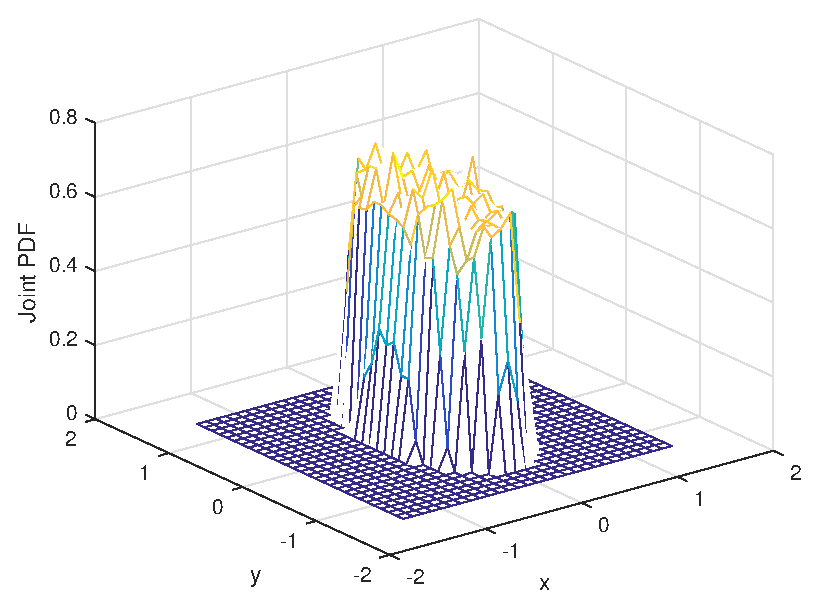
\includegraphics [width=4in]{prob_5_79_01.eps}



\end{document}
    
